\documentclass{standalone}
\usepackage{tikz}
\begin{document}
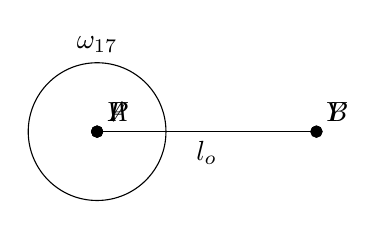
\begin{tikzpicture}[scale=1.0]
  \filldraw (0.0, 0.0) circle (2pt) node[above right] {$P$};
  \filldraw (0.0, 0.0) circle (2pt) node[above right] {$A$};
  \filldraw (0.0, 0.0) circle (2pt) node[above right] {$V$};
  \filldraw (2.7856, 0.0) circle (2pt) node[above right] {$Y$};
  \filldraw (2.7856, 0.0) circle (2pt) node[above right] {$B$};
  \draw (0.0, 0.0) -- (2.7856, 0.0) node[midway, below] {$l_o$};
  \draw (0.0, 0.0) circle (0.8747) node[above=0.8747cm] {$\omega_{17}$};
\end{tikzpicture}
\end{document}